\Transcb{yellow}{blue}{Search for a diffuse cosmic $\nu$ flux}
\twocolumn
\vspace*{5mm}
%
\begin{itemize}
\item Many point sources : diffuse $\nu$ flux
\item[] Expected flux $\sim E^{-2}$
\item[] (Fermi shock acceleration)
\item[] Observed in TeV photons
\item CR primaries : flux $\sim E^{-2.7}$
\item[] $\rightarrow$ Calculate atm. $\nu$ $E$-spectrum
\item IceCube observed atm. $\nu$ spectrum
\item[] Validate calculated spectrum
\item[$\ast$] {\blue PDF for atm. $\nu$ $E$-spectrum}
\item Energy determination is essential
\item[] \colorbox{yellow}{Require contained events}
\end{itemize}

\newpage 
%
%\vspace*{5mm}
\begin{center}
{\blue The atmospheric neutrino spectrum}\\
(ICRC2013)\\
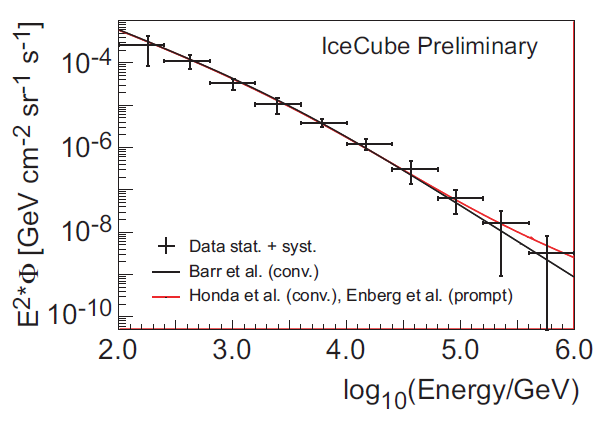
\includegraphics[keepaspectratio,width=13cm]{atm-nu}
\end{center}
%
\begin{itemize}
\item Very high E : Nearly atm. bkg free
\item[] 0.1 atm. $\nu$ per year at 1 PeV
\item[] \colorbox{yellow}{EHE events might prove cosmic $\nu$}
\end{itemize}

\Tr
\begin{center}
{\blue Tue 09-aug-2011 07:23:18 UTC}\\
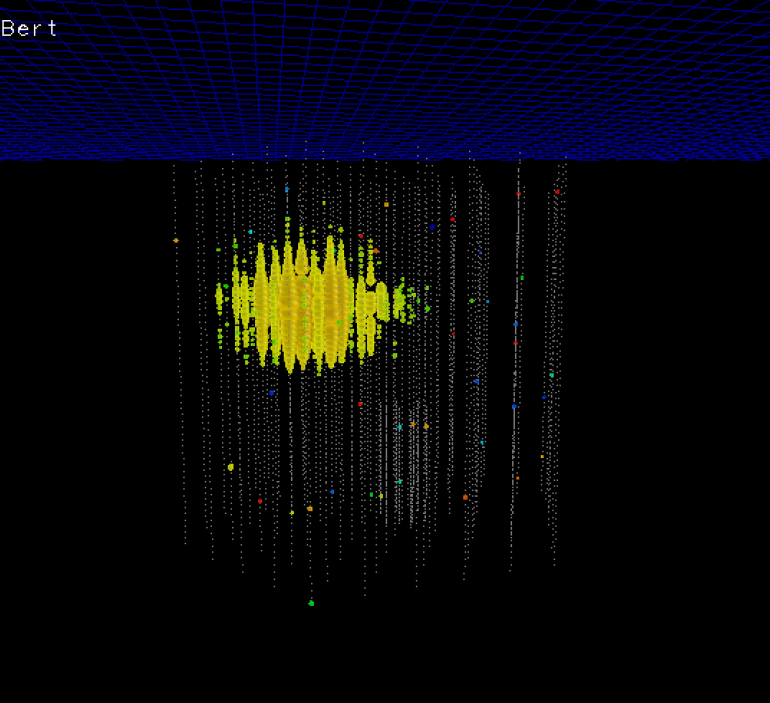
\includegraphics[keepaspectratio,width=13cm]{bert}\\
$1.04 \pm 0.14$ PeV
\end{center}
{\blue Atmospheric $\nu$ background ?}

\newpage

\begin{center}
{\blue Tue 03-jan-2012 03:34:01 UTC}\\
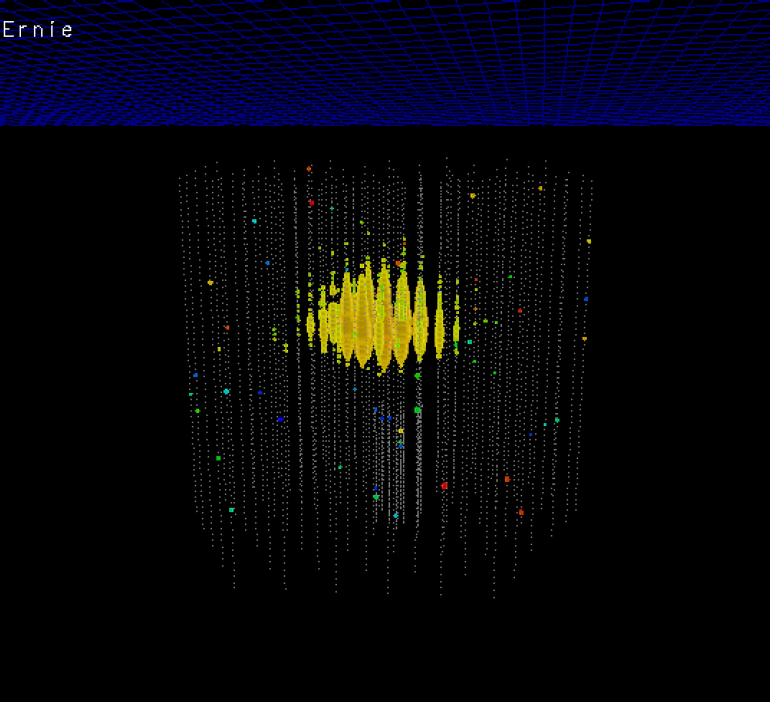
\includegraphics[keepaspectratio,width=13cm]{ernie}\\
$1.14 \pm 0.14$ PeV
\end{center}
{\blue P-value : $2.9 \cdot 10^{-3} \quad (2.8 \sigma)$}

\Tr
\onecolumn
\begin{center}
{\blue Try to get more "Muppets in the basket"}
\end{center}
%
\begin{itemize}
\item Perform a High-Energy Starting Event analysis (may 2010$-$may 2013)
\item[] Use event start veto criteria $\rightarrow$ remove atm. bkg $\mu$ and $\nu$ (showers)
\item[] Guarantees (contained) $\nu$ events and allows lower $E$ cut $\rightarrow 4\pi$
\end{itemize}
%
\begin{center}
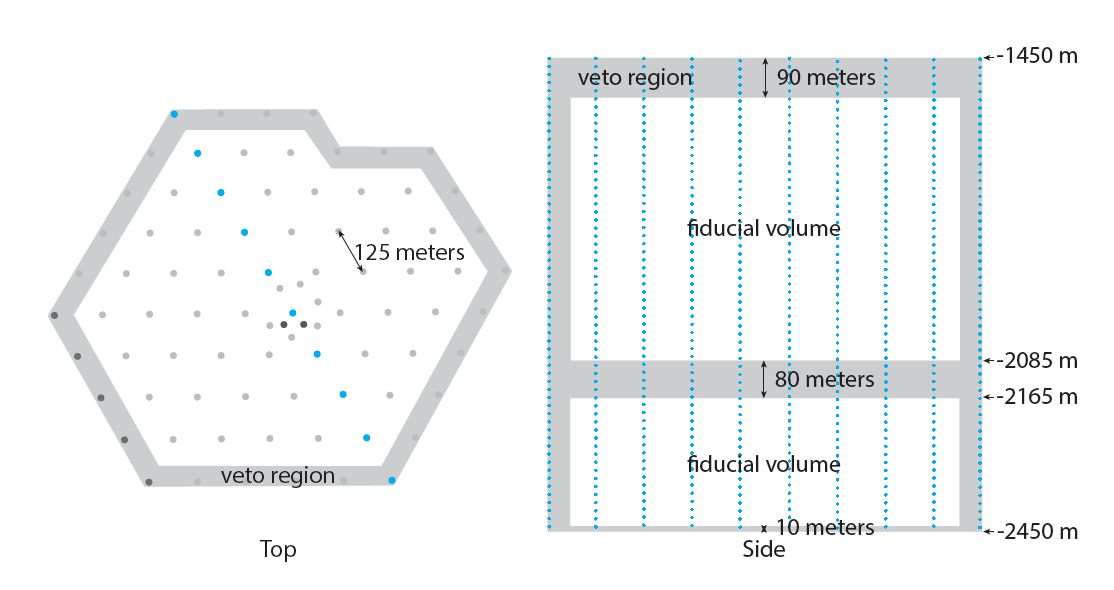
\includegraphics[keepaspectratio,height=10cm]{veto}
\end{center}

\Tr
\twocolumn[\begin{center}{\blue 35 additional events were found}\end{center}]
%
\begin{center}
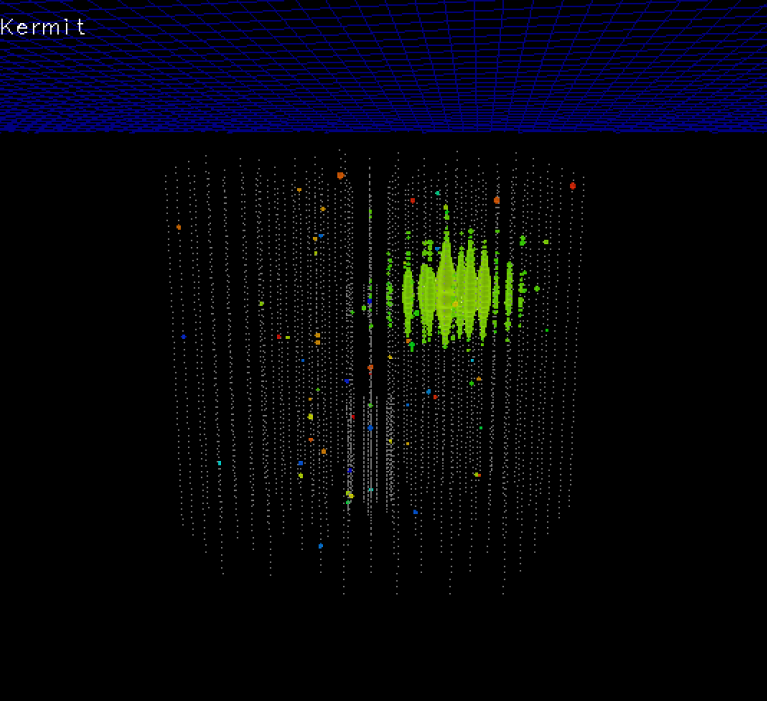
\includegraphics[keepaspectratio,width=13cm]{kermit}
\end{center}

\newpage

\begin{center}
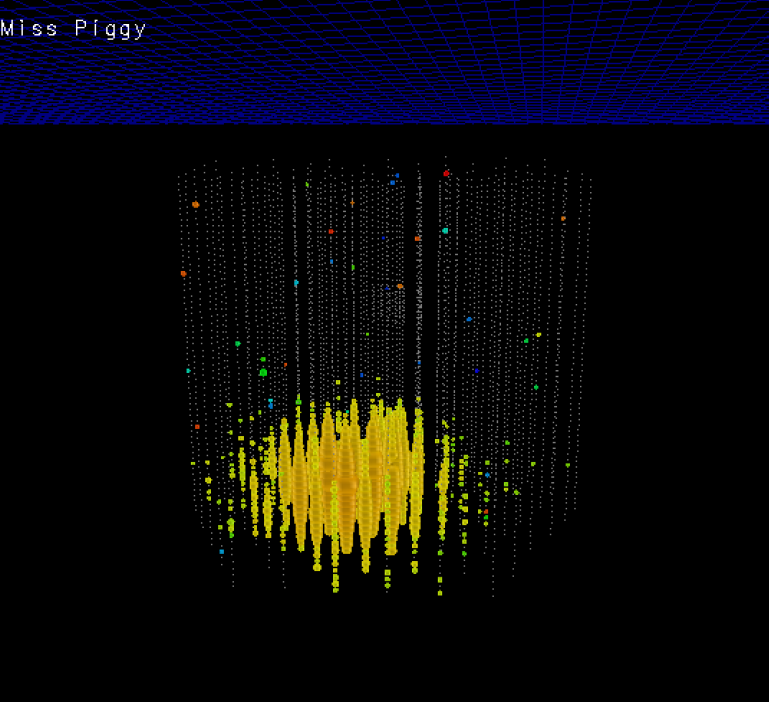
\includegraphics[keepaspectratio,width=13cm]{miss-piggy}
\end{center}

\Tr
\twocolumn[\begin{center}{\blue Also some $\mu$ track signatures}\end{center}]
%
\begin{center}
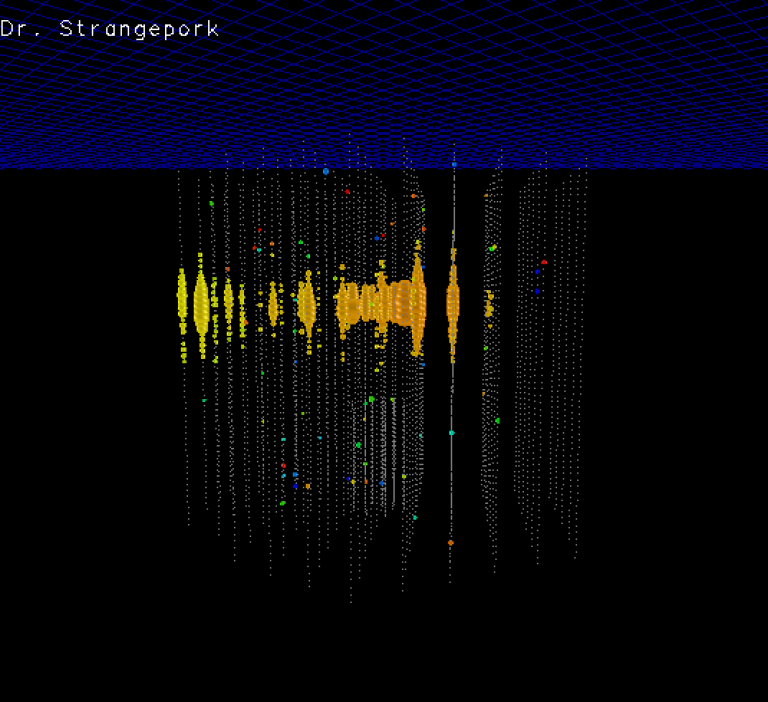
\includegraphics[keepaspectratio,width=13cm]{dr-strangepork}
\end{center}

\newpage

\begin{center}
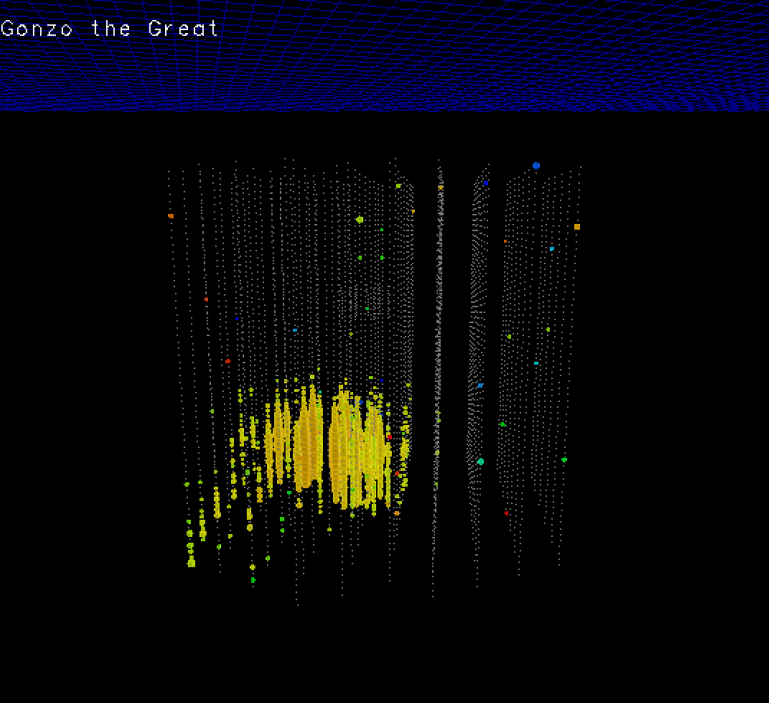
\includegraphics[keepaspectratio,width=13cm]{gonzo-the-great}
\end{center}

\Tr
\twocolumn[\begin{center}{\blue Our current champion}\end{center}]
%
\begin{center}
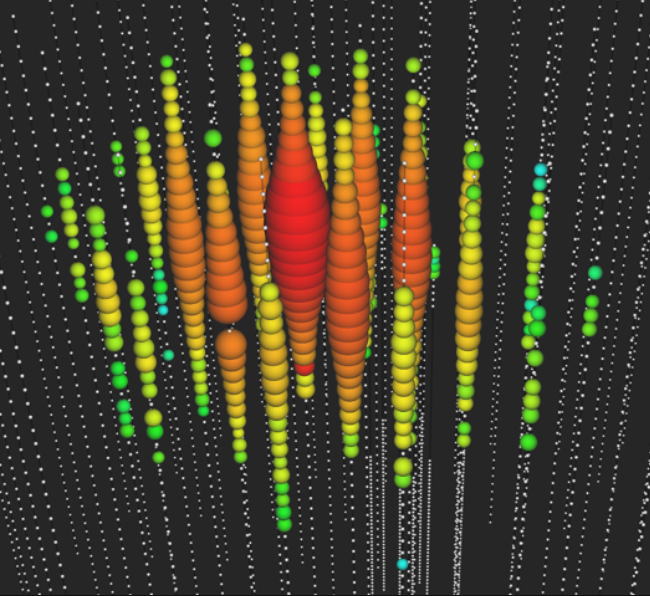
\includegraphics[keepaspectratio,width=13cm]{big-bird}\\
$2.00 \pm 0.25$ PeV
\end{center}

\newpage

\begin{center}

\includegraphics[keepaspectratio,height=12cm]{big-bird-photo}\\
Big Bird
\end{center}

\Tr
\onecolumn
\begin{center}
{\blue Energy distribution of the 37 events}
\end{center}
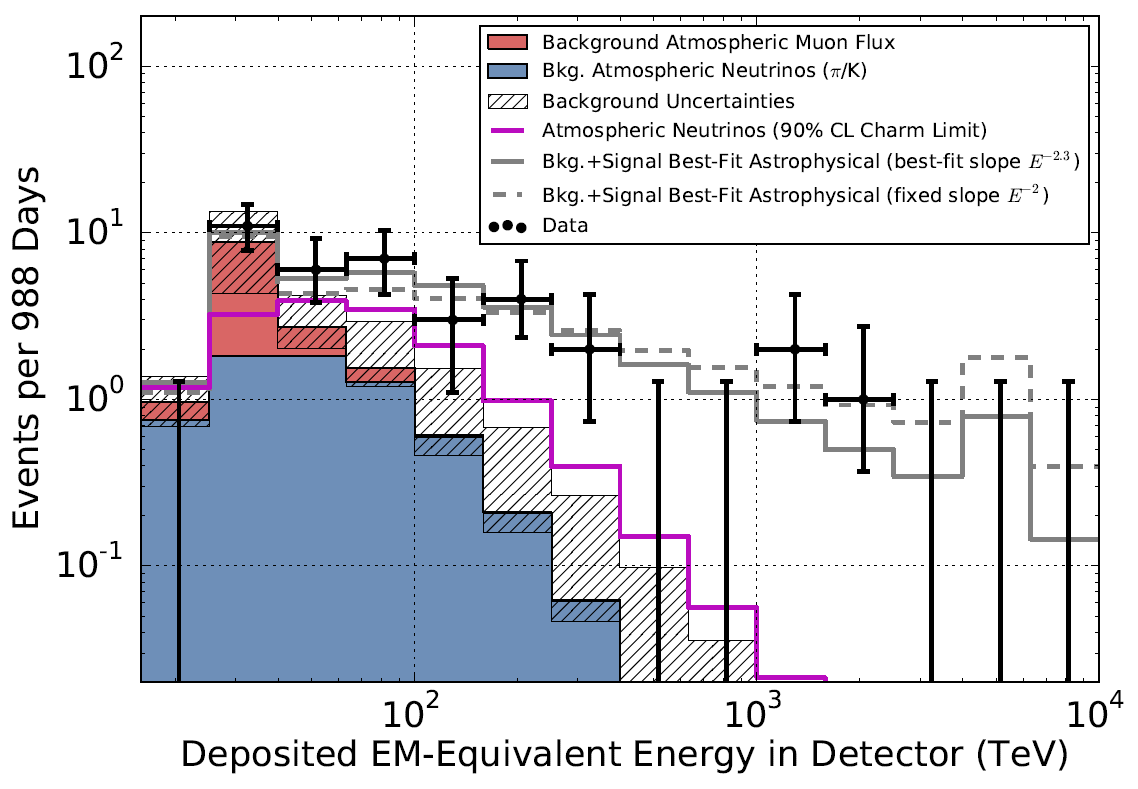
\includegraphics[keepaspectratio,width=13.5cm]{hese-e}
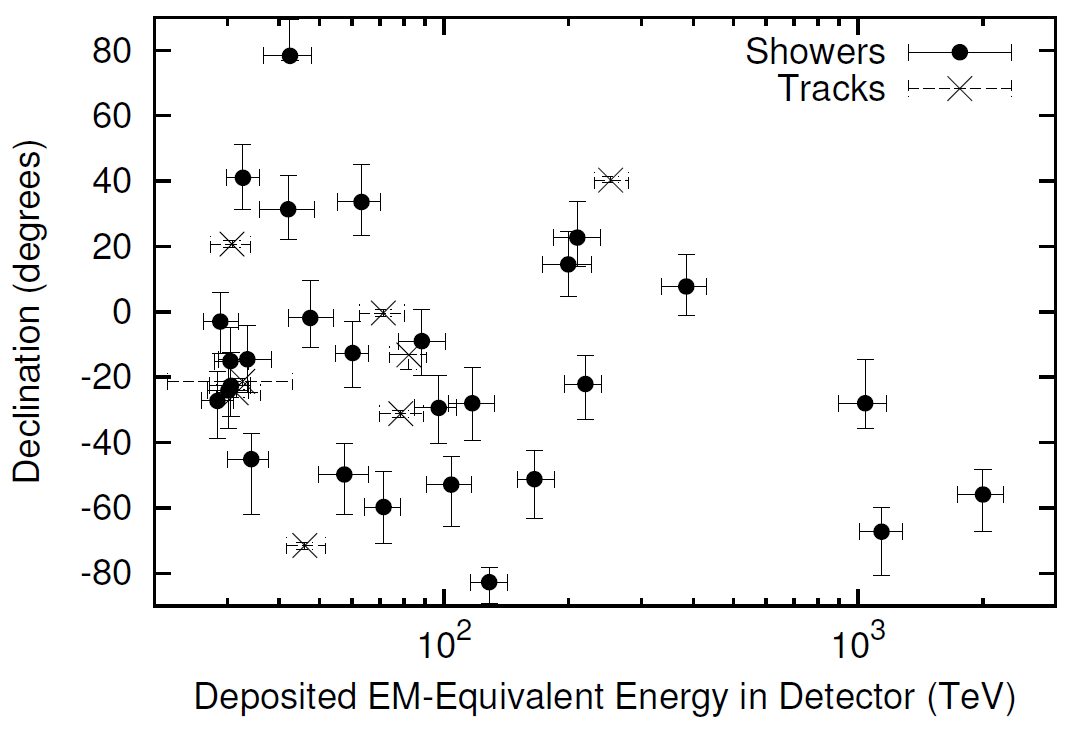
\includegraphics[keepaspectratio,width=13.5cm]{hese-decl-vs-e}
\begin{center}
\colorbox{yellow}{Evidence for cosmic high-energy neutrinos}
\end{center}

\Tr
\onecolumn
\begin{center}
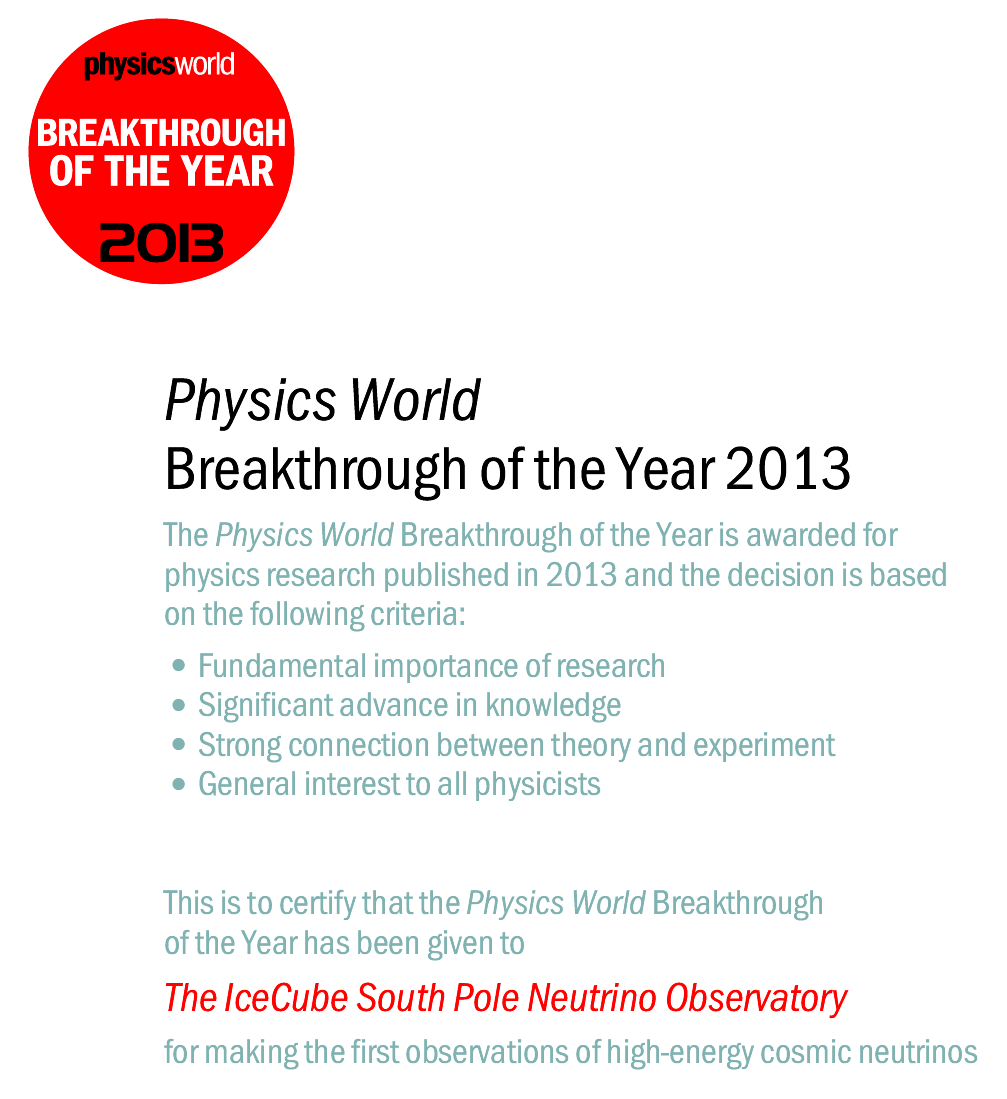
\includegraphics[keepaspectratio,height=15cm]{breakthrough}\\
\end{center}

\Tr
\onecolumn
\begin{center}
{\blue Cosmic origin confirmed at lower energies}\\[5mm]
{\red IceCube Preliminary}\\
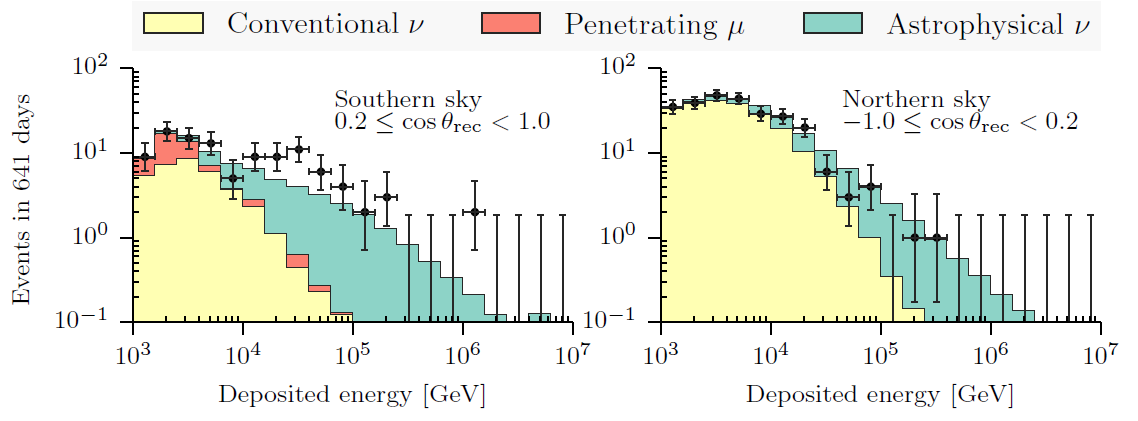
\includegraphics[keepaspectratio,width=25cm]{mese}\\[1cm]
\colorbox{yellow}{IceCube has raised the curtain for Neutrino Astronomy}
\end{center}

\Tr
\onecolumn
\begin{center}
{\blue Source directions of the 37 events}\\
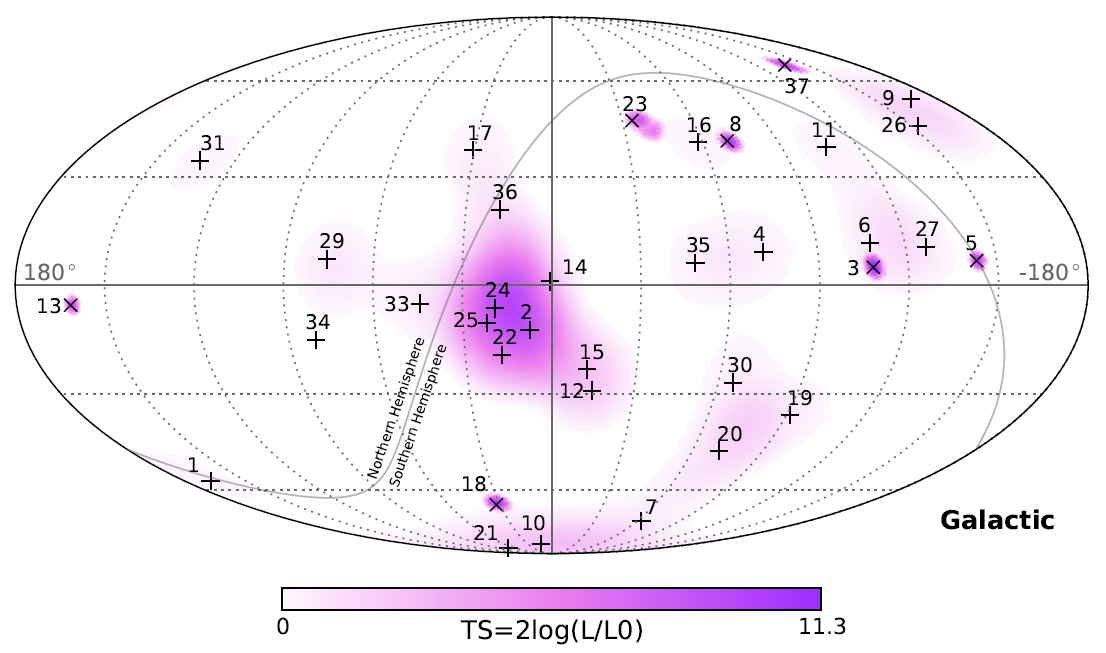
\includegraphics[keepaspectratio,width=20cm]{hese-skymap-gal}\\
\colorbox{yellow}{No evidence for point source(s)}
\end{center}

\Tr
\twocolumn
%
\begin{center}
{\blue The IceCube observed CR anisotropy}\\
(ApJ 740 (2011) 16)\\
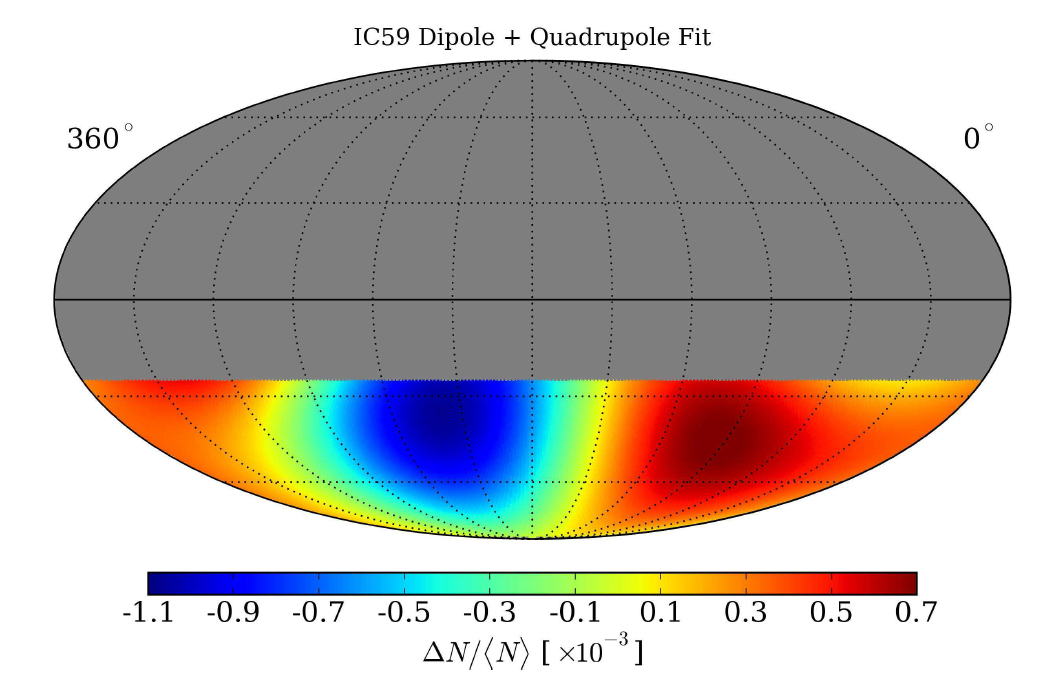
\includegraphics[keepaspectratio,width=13cm]{cr-anisotropy}\\[5mm]
\end{center}

\newpage

\begin{center}
{\blue The skymap of our 37 events}\\[1.2cm]
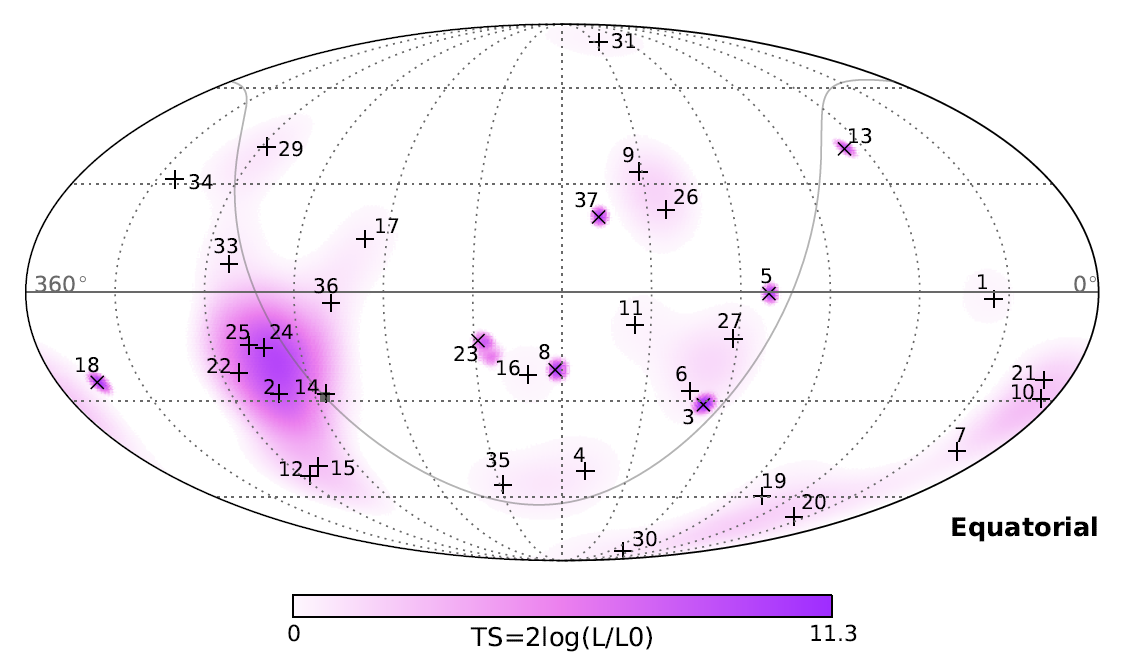
\includegraphics[keepaspectratio,width=13cm]{hese-skymap-equ}\\[5mm]
Investigating correlations might become interesting
\end{center}
